\section{"ЛУЧШИЕ УЗЛЫ. ПОДБОРКА ОТ АНАЛИТИКА".- Романенко Е.А..- v3.0, 21.08.2019}

Книга представляет собой подборку небольшого числа узлов, которые, по мнению автора, могут найти наиболее частое применение.

\graphicspath{{\currentpath}}

\subsection{Классификация узлов, предложенная автором}

\begin{enumerate}
\item Соединительные узлы
\begin{enumerate}
\item Легкоразвязываемые соединительные узлы.
Внутри автор выделяет регулируемые узлы
\item Условно-развязываемые соединительные узлы
Часть узлов этой группы автор выделил в "УНИВЕРСАЛЬНЫЕ (любая верёвка/ЛЕСКА)"
\end{enumerate}
\item Петли
\begin{enumerate}
\item Срединные петли
\item Незатягивающиеся петли (концевые)
\begin{itemize}
\item БЫСТРОСБРОСЫ
\item ЛЕГКОРАЗВЯЗЫВАЕМЫЕ НП
\item УСЛОВНО-РАЗВЯЗЫВАЕМЫЕ НП
\item УНИВЕРСАЛЬНЫЕ НП (любая верёвка/ЛЕСКА)
\item ДВОЙНЫЕ НЕЗАТЯГИВАЮЩИЕСЯ ПЕТЛИ
\item Двойные условно-развязываемые НП
\end{itemize}
\item Регулируемые петли
\item Петли-защёлки
\item Затягивающиеся петли
\begin{itemize}
\item ДЛЯ ВЕРЁВКИ
\item УНИВЕРСАЛЬНЫЕ (любая верёвка/ЛЕСКА)
\end{itemize}
\item Петли-удавки
\end{enumerate}
\item Крепёжные узлы (вяжутся вокруг Опоры)
Внутри автор выделяет
\begin{itemize}
\item ШТЫКИ
\item ОБЖИМНЫЕ / СТЯГИВАЮЩИЕ
\item УЗЛЫ ДЛЯ КОЛЬЦА («RING HITCHES») – [рин-хичи]
\item СХВАТЫВАЮЩИЕ УЗЛЫ
\item *БУКСИРОВОЧНЫЕ* УЗЛЫ
\end{itemize}
Но список ими не исчерпывается.
\item ОСОБЫЕ УЗЛЫ
\begin{itemize}
\item РЕВЕРСНО-СБРАСЫВАЕМЫЕ УЗЛЫ, или [САМОСБРОСЫ]
\item ПОЛИСПАСТЫ
\item Стопорные узлы, или [узлы для утолщения троса]
\item РАЗНОЕ - сюда автор включил гачные, бочечные, "досочные" и другие узко специализированные узлы
\end{itemize}
Кроме того вне подгрупп идёт амфорный узел.
\end{enumerate}

\subsection{Операции перобразования узлов, введённые автром}

\begin{enumerate}
\item СПРЯМЛЕНИЕ  – процедура, превращающая Травяной узел в Прямой. 
\item РЕВЕРСИРОВАНИЕ  – технически, это не узловязочная операция, это метод создания нового узла, и заключается он в том, что ходовой и коренной концы верёвки (одной или обеих) меняются "должностями".
\item ИНВЕРТИРОВАНИЕ (ходовых) или ИНВЕРСИЯ  – узловязочная операция, при которой ходовые концы на крайнем их пересечении меняются местами. Пример: взаимо-инвертируемы узлы Травяной и Тёщин 
\item СВИВКА - Из «хантера» при помощи свивки мы получаем Инфинити
\item операция, обратная спрямлению (автор названия не дал)
\end{enumerate}


Инверсия превращает
\begin{itemize}
\item Травяной - Тёщин
\item Узел Эшли(\#1452) - Скорняжный 
\item Альтер-С(\#1408) - \#1409
\item Хантер - Колобок Голдобина (сомнительно)
\item Одновитковый змеиный - Пропеллер (\#1421) (тоже сомнительно)
\end{itemize}


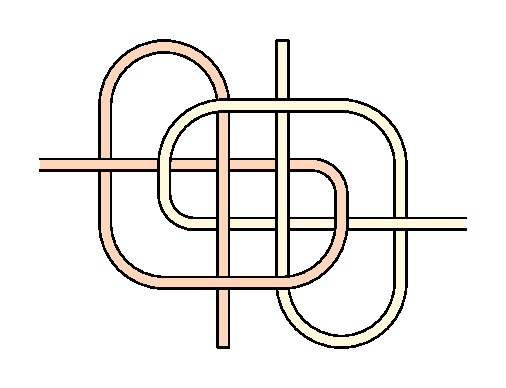
\includegraphics[scale=0.5]{images/hunter-bend.eps}
\includegraphics[scale=0.5]{images/kolobok-goldobina.eps}
\includegraphics[scale=0.5]{images/infinity.eps}


\subsection{Система именования узлов и их элементов, введённая автором}
Для обозначения узлов и их элементов автор использует систему сокращений:

\begin{tabular}{ll}
	ХК & Ходовой конец \\
	КК & Коренной конец \\
	ОО & Открытая опора \\
	ЗО & Закрытая опора \\
	КУ & Контрольный узел \\
	ПШ & Полуштык \\
	ИП & Исходное положение
\end{tabular}

\begin{tabular}{ll}
	СП & Срединная петля \\
	НП & Незатягивающаяся петля \\
	2НП & Двойная незатягивающаяся петля \\
	РП & Регулируемая петля \\
	ПЗ & Петля-зящёлка \\
	ПУ & Петля-удавка \\
	хич & Крепёжный узел \\
	РХ & Узел для кольца (ринг-хич) \\
	СУ & Схватывающий узел \\
	РСУ & Реверсно-сбрасываемый узел (самосброс) \\
	СтУ & Стопорный узел
\end{tabular}
